\documentclass[letterpaper]{article}
\usepackage[spanish,es-tabla]{babel}
\usepackage{indentfirst}
\usepackage{float}
\usepackage[utf8]{inputenc}
\usepackage{graphicx}

\begin{document}

\section{Ejercicio 3}

\begin{equation}
    x[n]=\delta[n]+\delta[n-1]+\delta[n-2]+\delta[n-3]
\end{equation}

\subsection{Calculo de la DTFT y la DFT}

Utilizando la definción de la DTFT:
\begin{equation}
    X(e^{j\omega})=\sum_{n=-\infty}^{\infty}x[n]e^{-j\omega n}
\end{equation}
Donde:
\begin{equation}
    \label{omega}
    \omega=2\pi f
\end{equation}
Llegamos a:
\begin{equation}
    \label{DTFT.R}
    X(e^{j\omega})=1+e^{-j\omega}+e^{-2j\omega}+e^{-3j\omega}
\end{equation}
Para el cálculo de la DFT utilizamos la ecuación:
\begin{equation}
    X[k]=\sum_{n=0}^{N-1}x[n]e^{-j\omega_k n}
\end{equation}
Donde:
\begin{equation}
    \label{omega.k}
    \omega_k=\frac{2\pi k}{N}
\end{equation}
Obteniendo:
\begin{equation}
    \label{DFT.R}
    X[k]=1+e^{\frac{-j2\pi k }{4}}+e^{\frac{-j4\pi k}{4}}+e^{\frac{-j6\pi k}{4}}
\end{equation}
Al comparar los resultados, ecuación \ref{DTFT.R} con ecuación \ref{DFT.R}, se observa que la diferencia recae en la frecuencia. Debido a esto, en la ecuación 
\ref{DTFT.R} la frecuencia asociada es la ecuación \ref{omega} que toma valores para todo $f$ dando como resultado un espectro continuo en frecuencia. Esto es un incoveniente a la hora 
de realizar el cálculo numérico (por los infinitos valores).Por esto para la \textit{DFT} se discretiza la frecuencia angular dando como resultado la ecuación \ref{omega.k}. Se concluye que es imposible encontrar de forma exacta la \textit{DTFT} a partir de la \textit{DFT}. En otras palabras, se puede decir que 
la \textit{DFT} muestrea el espectro continuo de la \textit{DTFT}.

\subsubsection{Calculo de la DFT con distintos puntos}    
Se generaron las señales con N=3, N=4 y N=8 y con dichas señales se calculo la DFT mediante la \textit{fft} y se obtuvieron los graficos presentando en la figura \ref{fig.3b}:

\begin{figure}[htb]
\centering
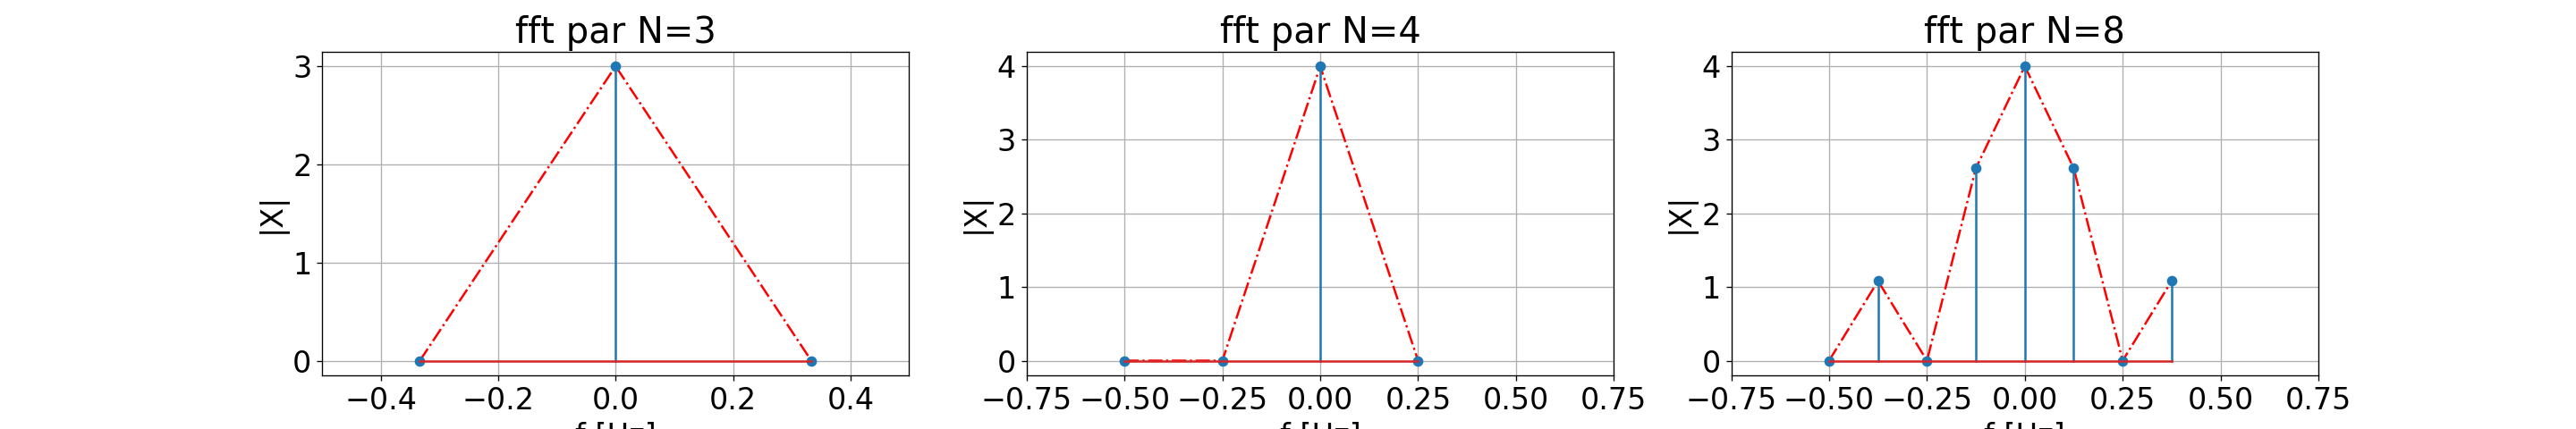
\includegraphics[width=\textwidth]{Img/punto_3_b.png}
\caption{Espectros generados con 3,4 y 8 puntos.}
\label{fig.3b}
\end{figure}

Se añadio en los graficos una señal punteada que corresponde al espectro real de la señal $x[n]$.
Se puede apreciar que los valores que toma la DFT coinciden con el valor de la envolvente en dichos puntos, por lo que seria posible aproximar la DTFT con la DFT.



\subsection{Calculo exacto de la DTFT}

    Para obtener la DTFT a partir de la \textit{fft}, la cual se puede asociar a un muestreo del espectro
    de la DTFT, mediante la siguiente relacion 

    \begin{equation}
        X[k]=X_{DTFT}\left(  \frac{2 \pi}{N} k \right)
    \end{equation}

    Donde $N$ es el numero de puntos que se utilizan para calcular la DFT.

    El calculo de la DTFT mediante el algoritmo de la \textit{fft} nunca sera exacto. Debido a que la DTFT es continua en frecuencia 
    mientras que la la DFT no. Pero los valores obtenido de la \textit{fft}, pueden ser considerados como muestras del espectro siempre que se 
    cumpla que 

    \begin{enumerate}
        \item Señal sea de duracion finita ($L$).
        \item Utilizar al menos $L$ puntos.
    \end{enumerate}
    


\end{document}